\chapter{Commentary}
\label{chap:commentary}
\typeout{START_CHAPTER "intro" \theabspage}

This document is an example of how to use the accompanying files
as well as some commentary on them.
The files are {\tt math\_commands.tex} and {\tt notation.tex}.
The file {\tt math\_commands.tex} includes several useful {\LaTeX}
macros and {\tt notation.tex } defines a notation page that could
be used at the front of any publication.

We developed these files while writing \citet{dlbook}.
We release these files for anyone to use freely, in order to help
establish some standard notation in the deep learning community.


\section{Examples}
\label{sec:examples}

We include this section as an example of some {\LaTeX} commands
and the macros we created for the book.

Citations that support a sentence without actually being used in the sentence
should appear at the end of the sentence using {\tt citep}:

\begin{quote}
Inventors have long dreamed of creating machines that think.
This desire dates back to at least the time of ancient Greece.
The mythical figures Pygmalion, Daedalus, and Hephaestus may
all be interpreted as legendary inventors, and
Galatea, Talos, and Pandora may all be regarded as artificial
life \citep{ovid2004metamorphoses,sparkes1996red,1997works}.
\end{quote}

When the authors of a document or the document itself are a noun in the
sentence, use the {\tt citet} command:

\begin{quote}
\citet{Mitchell:1997:ML} provides a succinct definition of machine learning:
``A computer program is said to learn from experience $E$ with respect to some
class of tasks $T$ and performance measure $P$, if its performance at tasks in
$T$, as measured by $P$, improves with experience $E$.''
\end{quote}

When introducing a new term, using the {\tt newterm} macro to highlight it.
If there is a corresponding acronym, put the acronym in parentheses
afterward. If your document includes an index, also use the {\tt index}
command.

\begin{quote}
Today, \newterm{artificial intelligence} (AI)\index{Artificial intelligence} is
a thriving field with many practical applications and active research topics.
\end{quote}

Sometimes you may want to make many entries in the index that all point
to a canonical index entry:

\begin{quote}
One of the simplest
and most common kinds of parameter norm penalty is
the squared $\normltwo$ parameter norm penalty
commonly known as \newterm{weight decay}.
\index{Weight decay}
In other academic communities,
$\normltwo$ regularization is also known as \newterm{ridge regression}
or \newterm{Tikhonov regularization}.
\index{Ridge regression|see {weight decay}}\index{Tikhonov regularization|see {weight decay}}
\end{quote}

To refer to a figure, use either {\tt figref} or {\tt Figref} depending on
whether you want to capitalize the resulting word in the sentence.

\begin{quote}
See \figref{fig:venn} for an example of a how to include graphics
in your document.
\Figref{fig:venn} shows how to include graphics in your document.
\end{quote}


\begin{figure}[t!]
\centering
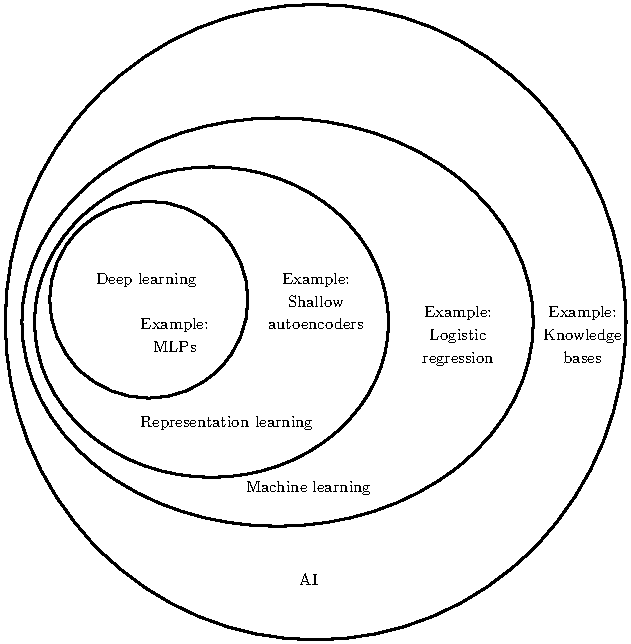
\includegraphics{venn}
\caption{An example of a figure.
The figure is a PDF displayed without being rescaled within {\LaTeX}.
The PDF was created at the right size to fit on the page, with the
fonts at the size they should be displayed. The fonts in the figure
are from the Computer Modern family so they match the fonts used
by \LaTeX.}
\label{fig:venn}
\end{figure}

Similarly, you can refer to different sections of the book using
{\tt partref}, {\tt Partref}, {\tt secref}, {\tt Secref}, etc.

\begin{quote}
	You are currently reading \secref{sec:examples}.
\end{quote}

\section*{Acknowledgments}
We thank Catherine Olsson and \'Ulfar Erlingsson for proofreading and
review of this manuscript.


\clearpage
%%
\typeout{END_CHAPTER "intro" \theabspage}
